% Fig 3.5 — Query2Doc generation pipeline

\documentclass[border=4pt]{standalone}
\usepackage{tikz}
\usetikzlibrary{positioning, arrows.meta, fit, backgrounds}

\begin{document}
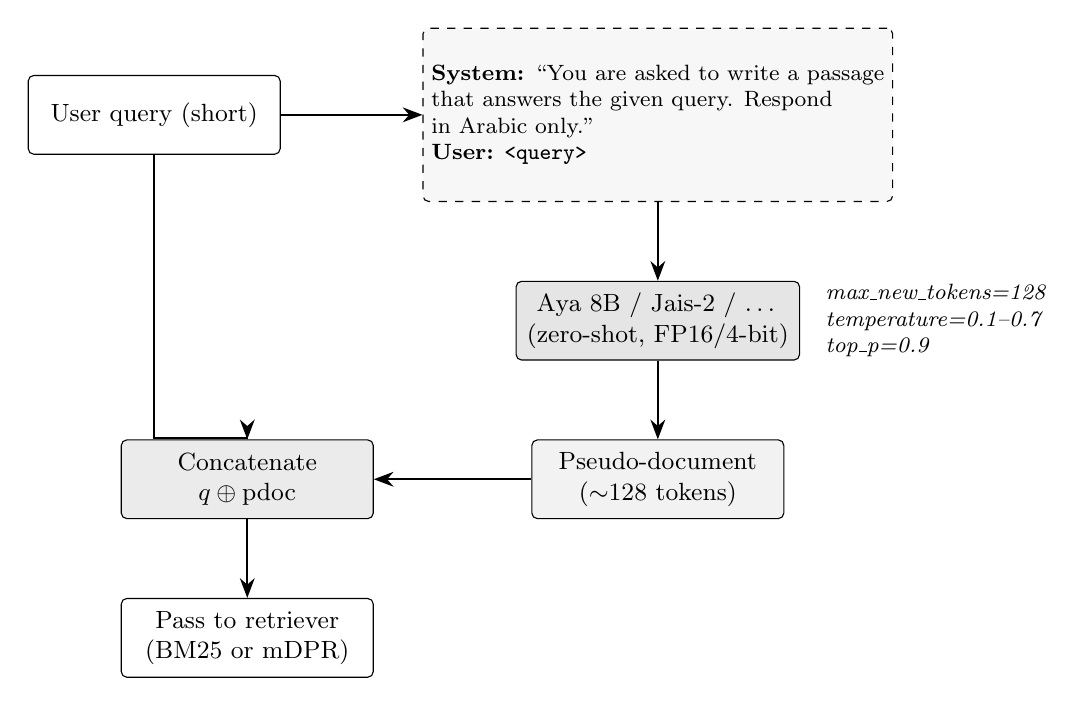
\begin{tikzpicture}[
    >=Stealth,
    node distance=10mm and 14mm,
    box/.style={rectangle, draw, rounded corners=2pt,
                minimum width=32mm, minimum height=10mm,
                align=center, font=\small},
    llm/.style={box, fill=black!10, minimum width=36mm},
    prompt/.style={rectangle, draw, dashed, rounded corners=2pt,
                   minimum width=58mm, minimum height=22mm,
                   align=left, font=\footnotesize, fill=black!3,
                   inner sep=3pt},
    data/.style={box, fill=black!5},
    arrow/.style={-{Stealth[length=2.5mm]}, thick}
]
  % Inputs
  \node[box] (q) {User query (short)};

  % Prompt template
  \node[prompt, right=of q, xshift=4mm] (tmpl)
    {\textbf{System:} ``You are asked to write a passage\\that answers the given query. Respond\\in Arabic only.''\\
     \textbf{User:} \texttt{<query>}};

  % LLM
  \node[llm, below=of tmpl] (llm) {Aya 8B / Jais-2 / \dots\\(zero-shot, FP16/4-bit)};

  % Pseudo-document
  \node[data, below=of llm] (pdoc) {Pseudo-document\\($\sim$128 tokens)};

  % Concatenation
  \node[box, fill=black!8, left=of pdoc, xshift=-6mm] (concat)
    {Concatenate\\$q \oplus \mathrm{pdoc}$};

  % Out to retriever
  \node[box, below=of concat] (retr) {Pass to retriever\\(BM25 or mDPR)};

  % Arrows
  \draw[arrow] (q.east) -- (tmpl.west);
  \draw[arrow] (tmpl) -- (llm);
  \draw[arrow] (llm) -- (pdoc);
  \draw[arrow] (pdoc) -- (concat);
  \draw[arrow] (q.south) -- ++(0, -36mm) -| (concat.north);
  \draw[arrow] (concat) -- (retr);

  % Generation params footnote
  \node[font=\footnotesize\itshape, right=2mm of llm.east, align=left]
    {max\_new\_tokens=128\\temperature=0.1--0.7\\top\_p=0.9};
\end{tikzpicture}
\end{document}
